\newpage
\section{Path}
\subsection{概述}

路径(path)是指一系列直线/曲线的片段集合。它对应的指令为 \textbackslash path。

\begin{lstlisting}[style = latex]
    \path <specification>
\end{lstlisting}

其中 <specification> 值一长串路径操作流,例如 (x,y) 坐标。在路径流中可以使用 [] 对路径进行修饰,用 {} 指定修饰范围。

\textbackslash path 指令虽然绘制了路径,但它并不会显示在图像上,需要使用 [draw] 修饰,通常使用 \textbackslash draw 或者 \textbackslash fill 指令替代 \textbackslash path 指令。

\begin{figure}[H]
    \centering
    \begin{minipage}{0.35\linewidth}
        \centering
        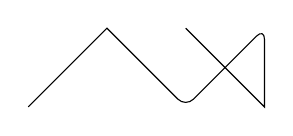
\begin{tikzpicture}[scale = 1]
            \draw (0,0) -- (1,1)
                [rounded corners] -- (2,0) -- (3,1)
                [sharp corners] -- (3,0) -- (2,1);
        \end{tikzpicture}
    \end{minipage}
    \begin{minipage}{0.55\linewidth}
        \begin{lstlisting}[style = latex-side]
    \draw (0,0) -- (1,1)
        [rounded corners] -- (2,0) -- (3,1)
        [sharp corners] -- (3,0) -- (2,1);
        \end{lstlisting}
    \end{minipage}
    \caption{Path:修饰}
\end{figure}

\begin{figure}[H]
    \centering
    \begin{minipage}{0.35\linewidth}
        \centering
        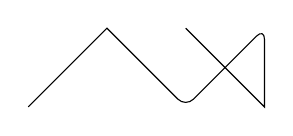
\begin{tikzpicture}[scale = 1]
            \draw (0,0) -- (1,1) 
                {[rounded corners] -- (2,0) -- (3,1)}
                -- (3,0) -- (2,1);
        \end{tikzpicture}
    \end{minipage}
    \begin{minipage}{0.55\linewidth}
        \begin{lstlisting}[style = latex-side]
    \draw (0,0) -- (1,1) 
        {[rounded corners] -- (2,0) -- (3,1)}
        -- (3,0) -- (2,1);
        \end{lstlisting}
    \end{minipage}
    \caption{Path:范围}
\end{figure}

有些修饰无论在何处给出,都会影响整个路径。一种解决方法是写多个路径。

\begin{figure}[H]
    \centering
    \begin{minipage}{0.35\linewidth}
        \centering
        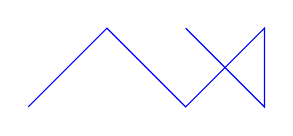
\begin{tikzpicture}[scale = 1]
            \draw (0,0) -- (1,1)
                [color=red] -- (2,0) -- (3,1)
                [color=blue] -- (3,0) -- (2,1);
        \end{tikzpicture}
    \end{minipage}
    \begin{minipage}{0.55\linewidth}
        \begin{lstlisting}[style = latex-side]
    \draw (0,0) -- (1,1)
        [color=red] -- (2,0) -- (3,1)
        [color=blue] -- (3,0) -- (2,1);
        \end{lstlisting}
    \end{minipage}
    \caption{Path:全局修饰}
\end{figure}

值得注意的是,Node 并不是 Path 的一部分,虽然 node 可以写在路径中,但逻辑上应该先绘制路径,再在路径周围添加节点。

下面解释一些常用的修饰。

\begin{itemize}
    \item name = <path name> 
    
    为路径命名,方便复用与定位。
    \item every path
    
    用于指定所有路径样式

    \begin{figure}[H]
        \centering
        \begin{minipage}{0.35\linewidth}
            \centering
            \begin{tikzpicture}[every path/.style = draw]
                \path (0,0) -- (1,0) -- (1,1) -- (0,1) -- cycle;
                \path (2,0) -- (2,1);
            \end{tikzpicture}
        \end{minipage}
        \begin{minipage}{0.55\linewidth}
            \begin{lstlisting}[style = latex-side]
    \begin{tikzpicture}[every path/.style = draw]
        \path (0,0) -- (1,0) -- (1,1) -- (0,1) -- cycle;
        \path (2,0) -- (2,1);
    \end{tikzpicture}
            \end{lstlisting}
        \end{minipage}
        \caption{Path:every path}
    \end{figure}

    \item insert path = <path>

    该修饰用于在路径上添加图形。它主要用于放置自定义图形。值得说明的是,最好不要将它用作节点。

    \begin{figure}[H]
        \centering
        \begin{minipage}{0.35\linewidth}
            \centering
            \begin{tikzpicture}[c/.style = {insert path = {circle[radius = 2pt]}}]
                \draw (0,0) -- (1,1)[c] -- (3,2)[c]; 
            \end{tikzpicture}
        \end{minipage}
        \begin{minipage}{0.55\linewidth}
            \begin{lstlisting}[style = latex-side]
    \begin{tikzpicture}[c./style = {insert path = {circle[radius = 2pt]}}]
        \draw (0,0) -- (1,1)[c] -- (3,2)[c]; 
    \end{tikzpicture}
            \end{lstlisting}
        \end{minipage}
        \caption{Path:insert path}
    \end{figure}

    \item append after command = <path>
    
    在指令完成后执行。

    \begin{figure}[H]
        \centering
        \begin{minipage}{0.35\linewidth}
            \centering
            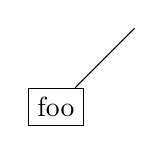
\begin{tikzpicture}[scale = 1]
                \draw node [append after command={(foo)--(1,1)},draw] (foo){foo};
            \end{tikzpicture}
        \end{minipage}
        \begin{minipage}{0.55\linewidth}
            \begin{lstlisting}[style = latex-side]
    \draw node [append after command={(foo)--(1,1)},draw] (foo){foo};
            \end{lstlisting}
        \end{minipage}
        \caption{Path:append after command}
    \end{figure}

    \item prefix after command = <path>
    
    与上一个修饰类似,不过它会在主路径绘制之后再绘制。
\end{itemize}

\subsection{路径绘制}
\subsubsection{直线绘制}
\noindent\textbf{基本语法}

直线绘制通过坐标点(coordinate)进行连线。其基本语法如下

\begin{lstlisting}[style = latex]
    \path ...<coordinate>...;
\end{lstlisting}

在一个命令中,直到;结尾之前,TikZ 允许进行多个同类路径绘制。

\begin{figure}[H]
    \centering
    \begin{minipage}{0.35\linewidth}
        \centering
        \begin{tikzpicture}[scale = 1]
            \draw (0,0) -- (2,0);
            \draw (0,1) -- (2,1);
        \end{tikzpicture}
    \end{minipage}
    \begin{minipage}{0.55\linewidth}
        \begin{lstlisting}[style = latex-side]
    \begin{tikzpicture}[scale = 1]
        \draw (0,0) -- (2,0);
        \draw (0,1) -- (2,1);
    \end{tikzpicture}
        \end{lstlisting}
    \end{minipage}
    \caption{Path:直线绘制}
\end{figure}

\noindent\textbf{路径闭合}

在绘制的路径过程中,往往要考虑起始点与终点的连接问题,其中一种方式是通过 (current subpath start) 可获得起始点的坐标,其效果等同于将起始点坐标写在最后。

\begin{figure}[H]
    \centering
    \begin{minipage}{0.35\linewidth}
        \centering
        
\begin{tikzpicture}[line width = 5pt]
            \draw (0,0) -- (1,0) -- (1,1) -- (0,1) -- (current subpath start);
        \end{tikzpicture}
    \end{minipage}
    \begin{minipage}{0.55\linewidth}
        \begin{lstlisting}[style = latex-side]
    
\begin{tikzpicture}[line width = 5pt]
        \draw (0,0) -- (1,0) -- (1,1) -- (0,1) -- (current subpath start);
    \end{tikzpicture}
        \end{lstlisting}
    \end{minipage}
    \caption{Path:current subpath start}
\end{figure}

在这个过程中发现衔接处并没有达到理想的处理效果,更常用的 cycle 可以解决这种闭合问题。

\begin{figure}[H]
    \centering
    \begin{minipage}{0.35\linewidth}
        \centering
        
\begin{tikzpicture}[line width = 5pt]
            \draw (0,0) -- (1,0) -- (1,1) -- (0,1) -- cycle;
        \end{tikzpicture}
    \end{minipage}
    \begin{minipage}{0.55\linewidth}
        \begin{lstlisting}[style = latex-side]
    
\begin{tikzpicture}[line width = 5pt]
        \draw (0,0) -- (1,0) -- (1,1) -- (0,1) -- cycle;
    \end{tikzpicture}
        \end{lstlisting}
    \end{minipage}
    \caption{Path:cycle}
\end{figure}

\noindent\textbf{垂线与水平线}

如果需要绘制垂线或水平线,可以使用 | - 两个关键字,分别代表垂线与水平线。在两点间使用 |- 代替 -- 意味着,先从第一个点出发,沿垂直方向到达第二个点的 y 坐标,再连接到第二个点,-| 同理。

\begin{figure}[H]
    \centering
    \begin{minipage}{0.35\linewidth}
        \centering
        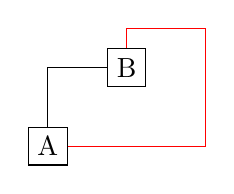
\begin{tikzpicture}[scale = 1]
            \draw (0,0) node(a) [draw] {A} (1,1) node(b) [draw] {B};
            \draw (a.north) |- (b.west);
            \draw[color=red] (a.east) -| (2,1.5) -| (b.north);
        \end{tikzpicture}
    \end{minipage}
    \begin{minipage}{0.55\linewidth}
        \begin{lstlisting}[style = latex-side]
    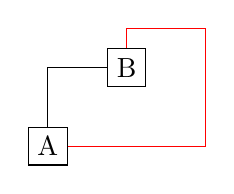
\begin{tikzpicture}[scale = 1]
        \draw (0,0) node(a) [draw] {A} (1,1) node(b) [draw] {B};
        \draw (a.north) |- (b.west);
        \draw[color=red] (a.east) -| (2,1.5) -| (b.north);
    \end{tikzpicture}
        \end{lstlisting}
    \end{minipage}
    \caption{Path:垂线与水平线}
\end{figure}

\subsubsection{曲线与圆角}

绘制曲线路径非常简单,在路径中加入 controls 语法即可。

\begin{figure}[H]
    \centering
    \begin{minipage}{0.35\linewidth}
        \centering
        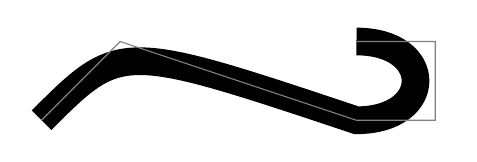
\begin{tikzpicture}[scale = 1]
            \draw[line width=10pt] (0,0) .. controls (1,1) .. (4,0)
                .. controls (5,0) and (5,1) .. (4,1);
            \draw[color=gray] (0,0) -- (1,1) -- (4,0) -- (5,0) -- (5,1) -- (4,1);
        \end{tikzpicture}
    \end{minipage}
    \begin{minipage}{0.55\linewidth}
        \begin{lstlisting}[style = latex-side]
    \draw[line width=10pt] (0,0) .. controls (1,1) .. (4,0)
        .. controls (5,0) and (5,1) .. (4,1);
    \draw[color=gray] (0,0) -- (1,1) -- (4,0) -- (5,0) -- (5,1) -- (4,1);
        \end{lstlisting}
    \end{minipage}
    \caption{Path:曲线}
\end{figure}

如果需要加入圆角,则可以使用上文已经提及的 rounded corners 修饰, 同时也可以为其指定圆角值。

\begin{figure}[H]
    \centering
    \begin{minipage}{0.35\linewidth}
        \centering
        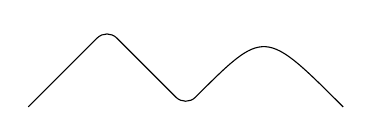
\begin{tikzpicture}[scale = 1]
            \draw [rounded corners = 5pt] (0,0) -- (1,1) -- (2,0) ..controls (3,1) .. (4,0);
        \end{tikzpicture}
    \end{minipage}
    \begin{minipage}{0.55\linewidth}
        \begin{lstlisting}[style = latex-side]
    \draw [rounded corners  = 5pt] (0,0) -- (1,1) -- (2,0) ..controls (3,1) .. (4,0); 
        \end{lstlisting}
    \end{minipage}
    \caption{Path:rounded corner}
\end{figure}

\subsection{常用图形绘制}
\subsubsection{矩形与网格}

绘制矩形的语法如下, rectangle 关键字左边的坐标为矩形一顶点,右边的坐标为另一顶点。
\begin{lstlisting}[style = latex]
    \path ...rectangle<corner or cycle>...;
\end{lstlisting}

\begin{figure}[H]
    \centering
    \begin{minipage}{0.35\linewidth}
        \centering
        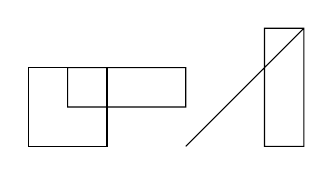
\begin{tikzpicture}[scale = 1]
            \draw (0,0) rectangle (1,1);
            \draw (.5,1) rectangle (2,0.5) (3,0) rectangle (3.5,1.5) -- (2,0);
        \end{tikzpicture}
    \end{minipage}
    \begin{minipage}{0.55\linewidth}
        \begin{lstlisting}[style = latex-side]
    \draw (0,0) rectangle (1,1);
    \draw (.5,1) rectangle (2,0.5) (3,0) rectangle (3.5,1.5) -- (2,0);
        \end{lstlisting}
    \end{minipage}
    \caption{Path:rectangle}
\end{figure}

网格的绘制语法与矩形类似:
\begin{lstlisting}[style = latex]
    \path ... grid[<options>]<corner or cycle> ...;
\end{lstlisting}

网格的常用修饰如下:
\begin{itemize}
    \item step = <number or dimension or coordinate> \hfill(默认:1cm)
    
    step 是网格最关键的修饰,决定了网格之间的间距。

    \begin{figure}[H]
        \centering
        \begin{minipage}{0.4\linewidth}
            \centering
            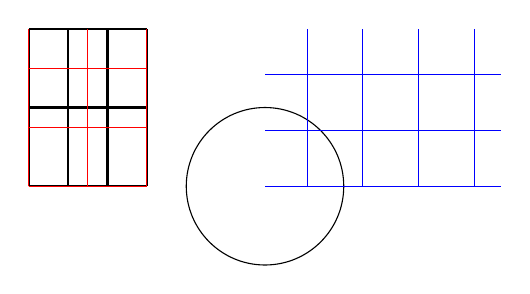
\begin{tikzpicture}[scale = 1]
                \begin{scope}[x=.5cm]
                    \draw[thick] (0,0) grid [step=1] (3,2);
                    \draw[red] (0,0) grid [step=.75cm] (3,2);
                \end{scope}
                \begin{scope}
                    \draw (3,0) circle [radius=1];
                    \draw[blue] (3,0) grid [step=(45:1)] (6,2);
                \end{scope}
            \end{tikzpicture}
        \end{minipage}
        \begin{minipage}{0.45\linewidth}
            \begin{lstlisting}[style = latex-side]
    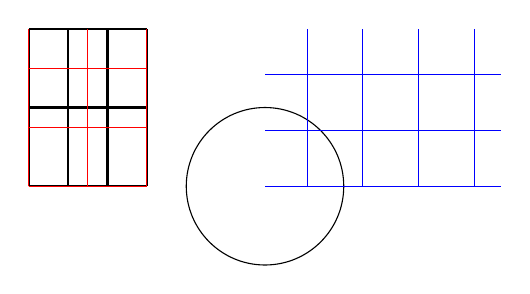
\begin{tikzpicture}[scale = 1]
        \begin{scope}[x=.5cm]
            \draw[thick] (0,0) grid [step=1] (3,2);
            \draw[red] (0,0) grid [step=.75cm] (3,2);
        \end{scope}
        \begin{scope}
            \draw (3,0) circle [radius=1];
            \draw[blue] (3,0) grid [step=(45:1)] (6,2);
        \end{scope}
    \end{tikzpicture}
            \end{lstlisting}
        \end{minipage}
        \caption{Path:grid-step}
    \end{figure}

    \item xstep/ystep = <dimension or number> \hfill(默认:1cm)
    
    用于控制 x 和 y 轴方向上的网格距离。

    \item help lines 
    
    TikZ 提供的一种网格类型,有修饰:[line width=0.2pt,gray]


\end{itemize}

\subsubsection{圆与椭圆}

绘制圆的语法如下,circle 关键字左边的坐标即为圆心。
\begin{lstlisting}[style = latex]
    \path ... circle[<options>] ...;
\end{lstlisting}

圆的常用修饰如下:
\begin{itemize}
    \item x radius = <value>
    
    指定水平方向半径,一般在定义椭圆时给出。
    \item y radius = <value>
    
    指定竖直方向半径,一般在定义椭圆时给出。
    \item radius = <value>
    
    指定圆半径。
    \item at = <coordinate>
    
    指定圆心位置。
\end{itemize}

\begin{figure}[H]
    \centering
    \begin{minipage}{0.35\linewidth}
        \centering
        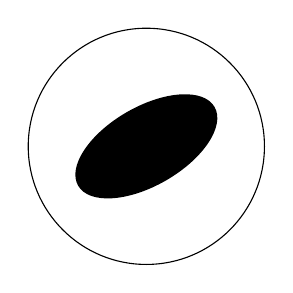
\begin{tikzpicture}[scale = 1]
            \draw (1,0) circle [radius=1.5];
            \fill (1,0) circle [x radius=1cm, y radius=5mm, rotate=30];
        \end{tikzpicture}
    \end{minipage}
    \begin{minipage}{0.55\linewidth}
        \begin{lstlisting}[style = latex-side]
    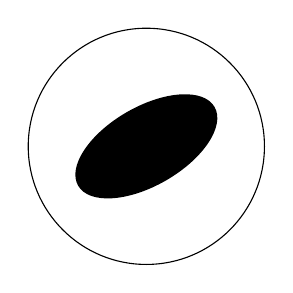
\begin{tikzpicture}[scale = 1]
        \draw (1,0) circle [radius=1.5];
        \fill (1,0) circle [x radius=1cm, y radius=5mm, rotate=30];
    \end{tikzpicture}
        \end{lstlisting}
    \end{minipage}
    \caption{Path:circle}
\end{figure}

椭圆语法如下:
\begin{lstlisting}[style = latex]
    \path … ellipse[hoptionsi] …;
\end{lstlisting}

其参数和圆几乎一致,圆可以通过 xradius/yradius 绘制成椭圆,那为什么要单独再定义一个关键字椭圆呢?原因是在类似 every circle/.style 等全局定义时可以进行区分。

\begin{figure}[H]
    \centering
    \begin{minipage}{0.35\linewidth}
        \centering
        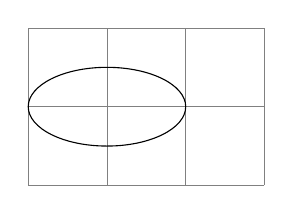
\begin{tikzpicture}[scale = 1]
            \draw [help lines] (0,0) grid (3,2);
            \draw (1,1) ellipse [x radius=1cm,y radius=.5cm];
        \end{tikzpicture}
    \end{minipage}
    \begin{minipage}{0.55\linewidth}
        \begin{lstlisting}[style = latex-side]
    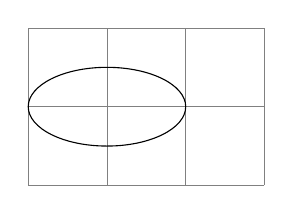
\begin{tikzpicture}[scale = 1]
        \draw [help lines] (0,0) grid (3,2);
        \draw (1,1) ellipse [x radius=1cm,y radius=.5cm];
    \end{tikzpicture}
        \end{lstlisting}
    \end{minipage}
    \caption{Path:ellipse}
\end{figure}

\subsubsection{弧线绘制}

绘制弧线的语法如下:
\begin{lstlisting}[style = latex]
    \path ... arc[<options>] ...;
\end{lstlisting}

弧线的常用修饰如下:
\begin{itemize}
    \item start angle = <degrees>
    
    设置弧线开始角度
    \item end angle = <degrees>
    
    设置弧线结束角度
    \item delta angle = <degrees>
    
    设置弧线变化角度
\end{itemize}

弧线的绘制默认以正x轴方向开始,按逆时针方向旋转。arc 关键字前的坐标,用于指定弧线的初始点位置,注意不是圆弧对应的中心。

\begin{figure}[H]
    \centering
    \begin{minipage}{0.35\linewidth}
        \centering
        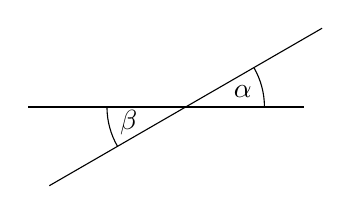
\begin{tikzpicture}[radius=1cm,delta angle=30]
            \draw (-1,0) -- +(3.5,0);
            \draw (1,0) ++(210:2cm) -- +(30:4cm);
            \draw (1,0) +(0:1cm) arc [start angle=0];
            \draw (1,0) +(180:1cm) arc [start angle=180];
            \path (1,0) ++(15:.75cm) node{$\alpha$};
            \path (1,0) ++(15:-.75cm) node{$\beta$};
        \end{tikzpicture}
    \end{minipage}
    \begin{minipage}{0.55\linewidth}
        \begin{lstlisting}[style = latex-side]
    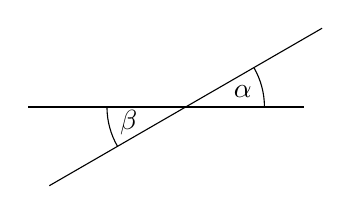
\begin{tikzpicture}[radius=1cm,delta angle=30]
        \draw (-1,0) -- +(3.5,0);
        \draw (1,0) ++(210:2cm) -- +(30:4cm);
        \draw (1,0) +(0:1cm) arc [start angle=0];
        \draw (1,0) +(180:1cm) arc [start angle=180];
        \path (1,0) ++(15:.75cm) node{$\alpha$};
        \path (1,0) ++(15:-.75cm) node{$\beta$};
    \end{tikzpicture}
        \end{lstlisting}
    \end{minipage}
    \caption{Path:arc}
\end{figure}

\subsection{数学函数绘制}
\subsubsection{抛物线}

绘制抛物线语法如下:
\begin{lstlisting}[style = latex]
    \path ...parabola[<options>]bend<bend coordinate><coordinate or cycle>...;
\end{lstlisting}

如果不使用 bend 关键字说明焦点坐标,则默认第一个点坐标为焦点坐标。

\begin{figure}[H]
    \centering
    \begin{minipage}{0.35\linewidth}
        \centering
        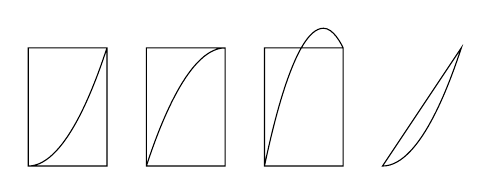
\begin{tikzpicture}[scale = 1]
            \draw (0,0) rectangle (1,1.5)
                  (0,0) parabola (1,1.5);
            \draw[xshift=1.5cm] (0,0) rectangle (1,1.5)
                  (0,0) parabola[bend at end] (1,1.5);
            \draw[xshift=3cm] (0,0) rectangle (1,1.5)
                  (0,0) parabola bend (.75,1.75) (1,1.5);
            \draw[xshift=4.5cm] (1,1.5) --
                  (0,0) parabola cycle;
        \end{tikzpicture}
    \end{minipage}
    \begin{minipage}{0.55\linewidth}
        \begin{lstlisting}[style = latex-side]
    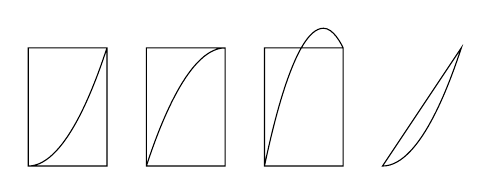
\begin{tikzpicture}[scale = 1]
        \draw (0,0) rectangle (1,1.5)
              (0,0) parabola (1,1.5);
        \draw[xshift=1.5cm] (0,0) rectangle (1,1.5)
              (0,0) parabola[bend at end] (1,1.5);
        \draw[xshift=3cm] (0,0) rectangle (1,1.5)
              (0,0) parabola bend (.75,1.75) (1,1.5);
        \draw[xshift=4.5cm] (1,1.5) --
              (0,0) parabola cycle;
    \end{tikzpicture}
        \end{lstlisting}
    \end{minipage}
    \caption{parabola}
\end{figure}

抛物线主要修饰如下:
\begin{itemize}
    \item bend = <coordinate>
    
    指明焦点坐标,在 [] 中语法为 [bend at <coordinate>],也可以写在 [] 外 bend <coordinate>。值得说明的是,如果指明的焦点与其他抛的点并不能构成抛物线,那么绘制的结果将不会是抛物线。
    \item bend pos = <fraction>
    
    用于指明焦点位置,需要配合 +<coordinate> 使用,以下面图形为例:
    \begin{figure}[H]
        \centering
        \begin{minipage}{0.35\linewidth}
            \centering
            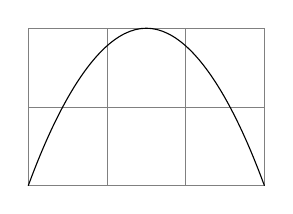
\begin{tikzpicture}[scale = 1]
                \draw[help lines] (0,0) grid (3,2);
                \draw (0,0) parabola[bend pos=0.5] bend +(0,2) +(3,0);
            \end{tikzpicture}
        \end{minipage}
        \begin{minipage}{0.55\linewidth}
            \begin{lstlisting}[style = latex-side]
    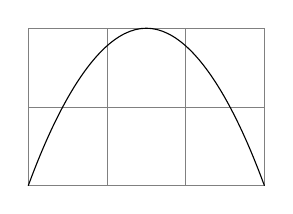
\begin{tikzpicture}[scale = 1]
        \draw[help lines] (0,0) grid (3,2);
        \draw (0,0) parabola[bend pos=0.5] bend +(0,2) +(3,0);
    \end{tikzpicture}
            \end{lstlisting}
        \end{minipage}
        \caption{Path:bend pos}
    \end{figure}

    bend pos = 0.5 指明了将曲线中点设置为焦点,紧随其后的 +(0,2) 和 +(3,0) 指明了该抛物线所占的矩形应为 2cm 高,3cm宽。
    \item parabola height = <dimension> 
    
    等效于:[bend pos=0.5,bend={+(0pt,<dimension>)}].
    \begin{figure}[H]
        \centering
        \begin{minipage}{0.35\linewidth}
            \centering
            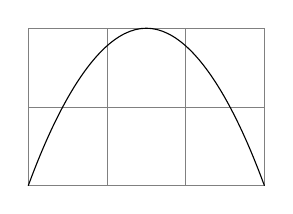
\begin{tikzpicture}[scale = 1]
                \draw[help lines] (0,0) grid (3,2);
                \draw (0,0) parabola[parabola height=2cm] +(3,0);
            \end{tikzpicture}
        \end{minipage}
        \begin{minipage}{0.55\linewidth}
            \begin{lstlisting}[style = latex-side]
    \draw[help lines] (0,0) grid (3,2);
    \draw (0,0) parabola[parabola height=2cm] +(3,0);
            \end{lstlisting}
        \end{minipage}
        \caption{Path:parabola height}
    \end{figure}

    \item bend at start/end
    
    将焦点放在起始点/终点。
\end{itemize}

\subsubsection{三角函数}

绘制三角函数的语法如下:

\begin{lstlisting}[style = latex]
    \path ... sin<coordinate or cycle> ...;
\end{lstlisting}

关键字 sin 左右边的坐标将作为区间 [$0,\pi/2$] 的端点对应的正弦函数坐标,绘制曲线。

\begin{figure}[H]
    \centering
    \begin{minipage}{0.35\linewidth}
        \centering
        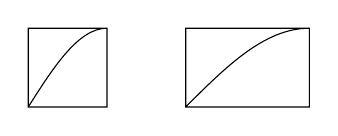
\begin{tikzpicture}[scale = 1]
            \draw (0,0) rectangle (1,1) (0,0) sin (1,1)
                  (2,0) rectangle +(1.57,1) (2,0) sin +(1.57,1);
        \end{tikzpicture}
    \end{minipage}
    \begin{minipage}{0.55\linewidth}
        \begin{lstlisting}[style = latex-side]
    \draw (0,0) rectangle (1,1) (0,0) sin (1,1)
        (2,0) rectangle +(1.57,1) (2,0) sin +(1.57,1);
        \end{lstlisting}
    \end{minipage}
    \caption{Path:sin}
\end{figure}

类似的,也有 cos 关键字,配合 cos 与 sin 关键字可以绘制出完整的三角函数图像。

\begin{figure}[H]
    \centering
    \begin{minipage}{0.35\linewidth}
        \centering
        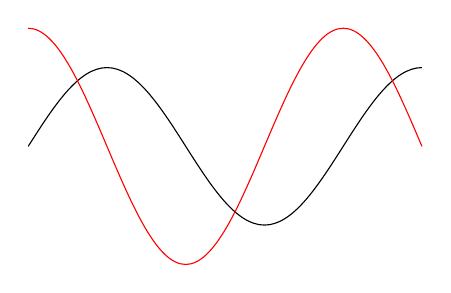
\begin{tikzpicture}[scale = 1]
            \draw            (0,0) sin (1,1) cos (2,0) sin (3,-1) cos (4,0) sin (5,1);
            \draw[color=red] (0,1.5) cos (1,0) sin (2,-1.5) cos (3,0) sin (4,1.5) cos (5,0);
        \end{tikzpicture}
    \end{minipage}
    \begin{minipage}{0.55\linewidth}
        \begin{lstlisting}[style = latex-side]
    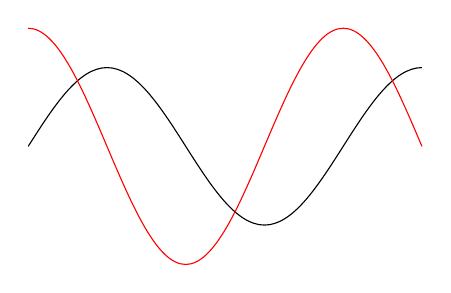
\begin{tikzpicture}[scale = 1]
        \draw (0,0) sin (1,1) cos (2,0) sin (3,-1) cos (4,0) sin (5,1);
        \draw[color=red] (0,1.5) cos (1,0) sin (2,-1.5) cos (3,0) sin (4,1.5) cos (5,0);
    \end{tikzpicture}
        \end{lstlisting}
    \end{minipage}
    \caption{Path:三角函数图像}
\end{figure}

\subsection{高阶操作}
\subsubsection{To Path 操作}

to 关键字的用法如下:

\begin{lstlisting}[style = latex]
    \path ... to[<options>]<nodes><coordinate or cycle> ...;
\end{lstlisting}

在默认情形下,to 与 -- 的效果相同,下文所介绍的修饰部分在 -- 关键字上也可以使用,但 to 关键字可以调用更多的修饰以达到更复杂的路径绘制效果。

\noindent\textbf{基础用法}

to 关键字的基础用法和 -- 类似。

\begin{figure}[H]
    \centering
    \begin{minipage}{0.35\linewidth}
        \centering
        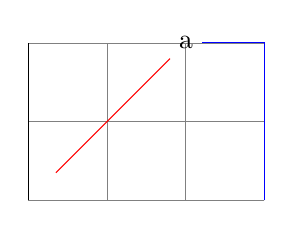
\begin{tikzpicture}[scale = 1]
            \draw[help lines] (0,0) grid (3,2);
            \node (a) at (2,2) {a};
            \draw (0,0) to (0,2);
            \draw[red] (10pt,10pt) to (a);
            \draw[blue] (3,0) -- (3,2) -- (a) -- cycle;
        \end{tikzpicture}
    \end{minipage}
    \begin{minipage}{0.55\linewidth}
        \begin{lstlisting}[style = latex-side]
    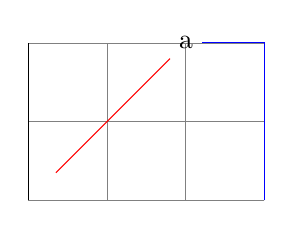
\begin{tikzpicture}[scale = 1]
        \draw[help lines] (0,0) grid (3,2);
        \node (a) at (2,2) {a};
        \draw (0,0) to (0,2);
        \draw[red] (10pt,10pt) to (a);
        \draw[blue] (3,0) -- (3,2) -- (a) -- cycle;
    \end{tikzpicture}
        \end{lstlisting}
    \end{minipage}
    \caption{Path:to}
\end{figure}

\noindent\textbf{to path 上的 Nodes}

在 to-path 路径上添加节点,与 -- 上语法一致。其中 out 和 in 分别表示起点出发方向与终点进入方向,是 to 关键字独有的语法。

\begin{figure}[H]
    \centering
    \begin{minipage}{0.35\linewidth}
        \centering
        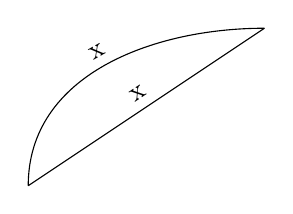
\begin{tikzpicture}
            \draw (0,0) to node [sloped,above] {x} (3,2);
            \draw (0,0) to[out=90,in=180] node [sloped,above] {x} (3,2);
        \end{tikzpicture}
    \end{minipage}
    \begin{minipage}{0.56\linewidth}
        \begin{lstlisting}[style = latex-side]
    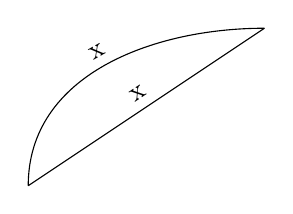
\begin{tikzpicture}
        \draw (0,0) to node [sloped,above] {x} (3,2);
        \draw (0,0) to[out=90,in=180] node [sloped,above] {x} (3,2);
    \end{tikzpicture}
        \end{lstlisting}
    \end{minipage}
    \caption{Path:to-node}
\end{figure}

由上例可以看出,添加 node 往往使得语句可读性下降,TikZ 还提供了将 node 写在 to 修饰中的语法,其几个常用修饰如下:

\begin{itemize}
    \item edge node = <node specification>
    
    该修饰可用于将 node 节点写在 to 的修饰中。
    \begin{figure}[H]
        \centering
        \begin{minipage}{0.35\linewidth}
            \centering
            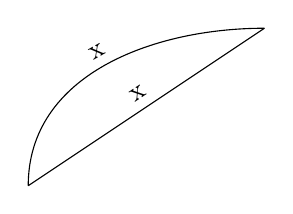
\begin{tikzpicture}[scale = 1]
                \draw (0,0) to [edge node={node [sloped,above] {x}}] (3,2);
                \draw (0,0) to [out=90,in=180,
                    edge node={node [sloped,above] {x}}] (3,2);
            \end{tikzpicture}
        \end{minipage}
        \begin{minipage}{0.55\linewidth}
            \begin{lstlisting}[style = latex-side]
    \draw (0,0) to [edge node={node [sloped,above] {x}}] (3,2);
    \draw (0,0) to [out=90,in=180,
        edge node={node [sloped,above] {x}}] (3,2);
            \end{lstlisting}
        \end{minipage}
        \caption{Path:edge node}
    \end{figure}

    \item edge label = <text>
    
    上文的语法还是比较复杂,在控制要求没那么严格的情况下,可以使用 edge label 修饰,它相当于 edge node={node[auto]{<text>}}.

    \item edge label' = <text>
    
    相当于:edge node={node[auto,swap]{<text>}}.

    \begin{figure}[H]
        \centering
        \begin{minipage}{0.35\linewidth}
            \centering
            \begin{tikzpicture}[scale = 1]
                \draw (0,0) to [edge label=x, edge label'=y] (3,2);
            \end{tikzpicture}
        \end{minipage}
        \begin{minipage}{0.55\linewidth}
            \begin{lstlisting}[style = latex-side]
    \draw (0,0) to [edge label=x, edge label'=y] (3,2);
            \end{lstlisting}
        \end{minipage}
        \caption{Path:edge label}
    \end{figure}

\end{itemize}

\noindent\textbf{全局样式}

TikZ 为 to 设置了 every to 修饰,这也是与 -- 关键字的另一区分。

\begin{figure}[H]
    \centering
    \begin{minipage}{0.35\linewidth}
        \centering
        \begin{tikzpicture}[every to/.style={append after command={[draw,dashed]}}]
            \draw (0,0) to (3,2);
        \end{tikzpicture}
    \end{minipage}
    \begin{minipage}{0.55\linewidth}
        \begin{lstlisting}[style = latex-side]
    \begin{tikzpicture}[every to/.style={append after command={[draw,dashed]}}]
        \draw (0,0) to (3,2);
    \end{tikzpicture}
        \end{lstlisting}
    \end{minipage}
    \caption{Path:every to}
\end{figure}

to path = <path> 可以辅助我们做一些路径微操。

\begin{itemize}
    \item to path 深入理解。
    
    每当 to 关键字起作用,就会创建一条对应的路径,在这个路径中会产生以下几个宏。
    \begin{itemize}
        \item \textbackslash tikztostart 起始点坐标
        \item \textbackslash tikztotarget 终点坐标
        \item \textbackslash tikztonodes 中间节点
    \end{itemize}

一个标准的包含 to 关键字的路径是由以下形式构成的
\begin{lstlisting}[style = latex]
    -- (\tikztotarget) \tikztonodes
\end{lstlisting}

我可以修改上述的 path 形式

\begin{figure}[H]
    \centering
    \begin{minipage}{0.35\linewidth}
        \centering
        \begin{tikzpicture}[to path={
            .. controls +(1,0) and +(1,0) .. (\tikztotarget) \tikztonodes}]
            \node (a) at (0,0) {a};
            \node (b) at (2,1) {b};
            \node (c) at (1,2) {c};
            \draw (a) to node {x} (b)
                  (a) to (c);
        \end{tikzpicture}
    \end{minipage}
    \begin{minipage}{0.55\linewidth}
        \begin{lstlisting}[style = latex-side]
    \begin{tikzpicture}[to path={
        .. controls +(1,0) and +(1,0) .. (\tikztotarget) \tikztonodes}]
        \node (a) at (0,0) {a};
        \node (b) at (2,1) {b};
        \node (c) at (1,2) {c};
        \draw (a) to node {x} (b)
              (a) to (c);
    \end{tikzpicture}
        \end{lstlisting}
    \end{minipage}
    \caption{Path:to path}
\end{figure}

我们也可以自定义自己的 path 样式

\tikzset{
    my loop/.style={to path={
    .. controls +(80:1) and +(100:1) .. (\tikztotarget) \tikztonodes}},
    my state/.style={circle,draw}
}

\begin{figure}[H]
    \centering
    \begin{minipage}{0.35\linewidth}
        \centering
        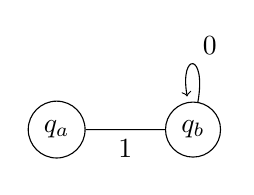
\begin{tikzpicture}[shorten >=2pt]
            \node [my state] (a) at (210:1) {$q_a$};
            \node [my state] (b) at (330:1) {$q_b$};
            \draw[->] (a) to node[below] {1} (b)
                to [my loop] node[above right] {0} (b);
        \end{tikzpicture}
    \end{minipage}
    \begin{minipage}{0.55\linewidth}
        \begin{lstlisting}[style = latex-side]
    \tikzset{
        my loop/.style={to path={
            .. controls +(80:1) and +(100:1) .. (\tikztotarget) \tikztonodes}},
        my state/.style={circle,draw}}

    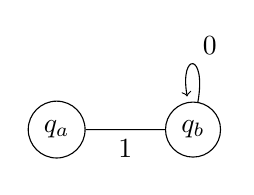
\begin{tikzpicture}[shorten >=2pt]
        \node [my state] (a) at (210:1) {$q_a$};
        \node [my state] (b) at (330:1) {$q_b$};
        \draw[->] (a) to node[below] {1} (b)
            to [my loop] node[above right] {0} (b);
    \end{tikzpicture}
        \end{lstlisting}
    \end{minipage}
    \caption{Path:自定义 to path}
\end{figure}

\item execute at begin to = <code>

在 at 之前执行 <code>
\item execute at end to = <code>

在 at 之后执行 <code>

\end{itemize}

\subsubsection{foreach 操作}

在 path 中使用 foreach 的语法如下:
\begin{lstlisting}[style = latex]
    \path ...foreach<variables>[<options>] in {<path commands>} ...;
\end{lstlisting}

\begin{figure}[H]
    \centering
    \begin{minipage}{0.35\linewidth}
        \centering
        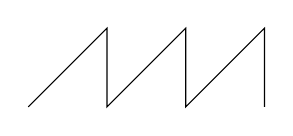
\begin{tikzpicture}[scale = 1]
            \draw (0,0) foreach \x in {1,...,3} { -- (\x,1) -- (\x,0) };
        \end{tikzpicture}
    \end{minipage}
    \begin{minipage}{0.55\linewidth}
        \begin{lstlisting}[style = latex-side]
    \draw (0,0) foreach \x in {1,...,3} { -- (\x,1) -- (\x,0) };
        \end{lstlisting}
    \end{minipage}
    \caption{Path:foreach}
\end{figure}

\subsubsection{Let 操作}

使用 let 关键字需要加载 calc 包,let 操作并不会拓展路径,主要起到辅助绘图作用,其语法如下。

\begin{lstlisting}[style = latex]
    \path ... let<assignment>,<assignment>,<assignment>... in ...;
\end{lstlisting}

在 <assignment> 中可以为坐标命名,以便整个语句中调用。具体的存储原理这里省略。

\begin{itemize}
    \item \textbackslash n {<number register>}
    
    这将存储一些数值,比如  \textbackslash n1 = {1pt+2pt} 再次调用  \textbackslash n1 时,将传值: 3pt。
    \item \textbackslash p<point register> = <coordinate>
    
    与 n 类似,\textbackslash p 用来保存坐标。
    \begin{figure}[H]
        \centering
        \begin{minipage}{0.35\linewidth}
            \centering
            \begin{tikzpicture}[scale = 1]
                \draw [help lines] (0,0) grid (3,2);
                \draw let \p{foo} = (1,1), \p2 = (2,0) in
                    (0,0) -- (\p2) -- (\p{foo});
            \end{tikzpicture}
        \end{minipage}
        \begin{minipage}{0.55\linewidth}
            \begin{lstlisting}[style = latex-side]
    \begin{tikzpicture}[scale = 1]
        \draw [help lines] (0,0) grid (3,2);
        \draw let \p{foo} = (1,1), \p2 = (2,0) in
            (0,0) -- (\p2) -- (\p{foo});
    \end{tikzpicture}
            \end{lstlisting}
        \end{minipage}
        \caption{Path:临时存储变量}
    \end{figure}

    \item \textbackslash x \textbackslash y 
    
    与上文 \textbackslash p 类似,但是仅存储 x 轴和 y 轴坐标。

    \begin{figure}[H]
        \centering
        \begin{minipage}{0.35\linewidth}
            \centering
            \begin{tikzpicture}
                \draw [help lines] (0,0) grid (3,2);
                \draw (1,0) coordinate (first point)
                    -- (3,2) coordinate (second point);
                \fill[red] let \p1 = (first point),
                               \p2 = (second point) in
                    (\x1,\y2) circle [radius=2pt];
            \end{tikzpicture}
        \end{minipage}
        \begin{minipage}{0.55\linewidth}
            \begin{lstlisting}[style = latex-side]
    \begin{tikzpicture}
        \draw [help lines] (0,0) grid (3,2);
        \draw (1,0) coordinate (first point)
            -- (3,2) coordinate (second point);
        \fill[red] let \p1 = (first point),
                       \p2 = (second point) in
            (\x1,\y2) circle [radius=2pt];
    \end{tikzpicture}
            \end{lstlisting}
        \end{minipage}
        \caption{Path:let 例子}
    \end{figure}

    \begin{figure}[H]
        \centering
        \begin{minipage}{0.35\linewidth}
            \centering
            \begin{tikzpicture}
                \draw [help lines] (0,0) grid (3,3);
                \coordinate (a) at (rnd,rnd);
                \coordinate (b) at (3-rnd,3-rnd);
                \draw (a) -- (b);
                \node (c) at (1,2) {x};
                \draw let \p1 = ($ (a)!(c)!(b) - (c) $),
                    \n1 = {veclen(\x1,\y1)}
                    in circle [at=(c), radius=\n1];
            \end{tikzpicture}
        \end{minipage}
        \begin{minipage}{0.55\linewidth}
            \begin{lstlisting}[style = latex-side]
    \begin{tikzpicture}
        \draw [help lines] (0,0) grid (3,3);
        \coordinate (a) at (rnd,rnd);
        \coordinate (b) at (3-rnd,3-rnd);
        \draw (a) -- (b);
        \node (c) at (1,2) {x};
        \draw let \p1 = ($ (a)!(c)!(b) - (c) $),
            \n1 = {veclen(\x1,\y1)}
            in circle [at=(c), radius=\n1];
    \end{tikzpicture}
            \end{lstlisting}
        \end{minipage}
        \caption{Path:let 例子2}
    \end{figure}

\end{itemize}

\subsubsection{路径存储}

上述的 \textbackslash p 仅能在一个语句内存储使用路径,如果需要在整个绘图环境中存储,则需要用到以下修饰。

\begin{itemize}
    \item save path = <macro>
    
    存储路径
    \item use path = <macro>
    
    使用已存储的路径
    \begin{figure}[H]
        \centering
        \begin{minipage}{0.35\linewidth}
            \centering
            \begin{tikzpicture}
                \path[save path=\pathA,name path=A] (0,1) to [bend left] (1,0);
                \path[save path=\pathB,name path=B]
                    (0,0) .. controls (.33,.1) and (.66,.9) .. (1,1);
                \fill[name intersections={of=A and B}] (intersection-1) circle (1pt);
                \draw[blue][use path=\pathA];
                \draw[red] [use path=\pathB];
            \end{tikzpicture}
        \end{minipage}
        \begin{minipage}{0.55\linewidth}
            \begin{lstlisting}[style = latex-side]
    \begin{tikzpicture}
        \path[save path=\pathA,name path=A] (0,1) to [bend left] (1,0);
        \path[save path=\pathB,name path=B]
            (0,0) .. controls (.33,.1) and (.66,.9) .. (1,1);
        \fill[name intersections={of=A and B}] (intersection-1) circle (1pt);
        \draw[blue][use path=\pathA];
        \draw[red] [use path=\pathB];
    \end{tikzpicture}
            \end{lstlisting}
        \end{minipage}
        \caption{Path:use path}
    \end{figure}

\end{itemize}

\subsection{拓展用法}
\subsubsection{SVG 操作}

svg 关键字可以让我们使用 svg 语法绘图,需要用到 svg.path 包。svg 在 TikZ 中的语法请查官方文档\footnote{后续可能会更新},这里只给出示例。

\begin{figure}[H]
    \centering
    \begin{minipage}{0.35\linewidth}
        \centering
        \begin{tikzpicture}[scale = 1]
            \filldraw [fill=red!20] (0,1) svg[scale=2] {h 10 v 10 h -10}
                node [above left] {upper left} -- cycle;
            \draw svg {M 0 0 L 20 20 h 10 a 10 10 0 0 0 -20 0};
        \end{tikzpicture}
    \end{minipage}
    \begin{minipage}{0.55\linewidth}
        \begin{lstlisting}[style = latex-side]
    \begin{tikzpicture}[scale = 1]
        \filldraw [fill=red!20] (0,1) svg[scale=2] {h 10 v 10 h -10}
            node [above left] {upper left} -- cycle;
        \draw svg {M 0 0 L 20 20 h 10 a 10 10 0 0 0 -20 0};
    \end{tikzpicture}
        \end{lstlisting}
    \end{minipage}
    \caption{Path:svg}
\end{figure}

\subsubsection{Plot 操作}

plot 关键字主要用于文件读取并绘制图像,语法请查官方文档。


\newpage